\documentclass{article}

\usepackage{fancyhdr}
\usepackage{extramarks}
\usepackage{amsmath}
\usepackage{amssymb}
\usepackage{amsthm}
\usepackage{amsfonts}
\usepackage{tikz}
\usepackage[plain]{algorithm}
\usepackage{algpseudocode}
\usepackage{lastpage}
\usepackage{caption}
\usepackage{subcaption}
\usepackage{nth}
\usetikzlibrary{automata,positioning,trees,dsp,chains,decorations.pathreplacing,angles,quotes,angles}
\usepackage[makeroom]{cancel}
\usepackage{mathtools}
\usepackage{listing}
\usepackage{color}
\usepackage[numbered,framed]{matlab-prettifier}
\usepackage{bold-extra}
\usepackage[T1]{fontenc} 
\usepackage{parskip}
\usepackage{gensymb}
\usepackage{siunitx}

%
% Basic Document Settings
%

\topmargin=-0.45in
\evensidemargin=0in
\oddsidemargin=0in
\textwidth=6.5in
\textheight=9.0in
\headsep=0.25in

\linespread{1.1}

\pagestyle{fancy}
\lhead{\hmwkAuthorName}
%\chead{\hmwkClass\ (\hmwkClassInstructor\hmwkClassTime): \hmwkTitle}
\chead{\hmwkClass\ : \hmwkTitle}
%\rhead{\firstxmark}
\rhead{\hmwkDueDate}
%\lfoot{\lastxmark}
\cfoot{\thepage\ of \pageref{LastPage}}

\renewcommand\headrulewidth{0.4pt}
\renewcommand\footrulewidth{0.4pt}

\setlength\parindent{0pt}

%
% Create Problem Sections
%

\newcommand{\enterProblemHeader}[1]{
    \nobreak\extramarks{}{Problem #1 continued on next page\ldots}\nobreak{}
    \nobreak\extramarks{Problem #1 (continued)}{Problem #1 continued on next page\ldots}\nobreak{}
}

\newcommand{\exitProblemHeader}[1]{
    \nobreak\extramarks{Problem #1 (continued)}{Problem #1 continued on next page\ldots}\nobreak{}
    \nobreak\extramarks{Problem #1}{}\nobreak{}
}

\newcounter{partCounter}
\nobreak\extramarks{Problem 1}{}\nobreak{}

%
% Homework Problem Environment
%
% This environment takes an optional argument. When given, it will adjust the
% problem counter. This is useful for when the problems given for your
% assignment aren't sequential. See the last 3 problems of this template for an
% example.
%
\newenvironment{homeworkProblem}[1][1]{
    \setcounter{secnumdepth}{0}
    \section{Problem #1}
    \enterProblemHeader{Problem #1}
}{
    \exitProblemHeader{\thesection}
}

%
% Homework Details
%   - Title
%   - Due date
%   - Due Time
%   - Class
%   - Section/Time
%   - Instructor
%   - Author
%

\newcommand{\hmwkTitle}{Problem Set Title}
\newcommand{\hmwkDueDate}{Due Date}
\newcommand{\hmwkClass}{ECE XXX}
\newcommand{\hmwkClassTime}{ 4:30 PM} % include a leading space if you choose to use this field (disabled for now)
\newcommand{\hmwkClassInstructor}{Instructor's Name} % (disabled for now)
\newcommand{\hmwkAuthorName}{\textbf{Student's Name}}

%
% Title Page
%


\title{
    \vspace{2in}
    \textmd{\textbf{\hmwkClass:\ \hmwkTitle}}\\
    \normalsize\vspace{0.1in}\small{Due\ on\ \hmwkDueDate}\\
    %\vspace{0.1in}\large{\textit{\hmwkClassInstructor\hmwkClassTime}}
    \vspace{2in}
}

\author{\hmwkAuthorName}
\date{}

\renewcommand{\part}[1]{\textbf{\large Part \Alph{partCounter}}\stepcounter{partCounter}\\}

%
% Various Helper Commands
%

% Useful for algorithms
\newcommand{\alg}[1]{\textsc{\bfseries \footnotesize #1}}

% For derivatives
\newcommand{\deriv}[1]{\frac{\mathrm{d}}{\mathrm{d}x} (#1)}

% For partial derivatives
\newcommand{\pderiv}[2]{\frac{\partial}{\partial #1} (#2)}

% Integral dx
\newcommand{\dx}{\mathrm{d}x}

% Alias for the Solution section header
\newcommand{\solution}{\textbf{\large Solution}}

% Probability commands: Expectation, Variance, Covariance, Bias
\newcommand{\E}[1]{\mathrm{E}\left[#1\right]}
\newcommand{\Var}[1]{\mathrm{Var}\left(#1\right)}
\newcommand{\Cov}[2]{\mathrm{Cov}\left(#1,#2\right)}
\newcommand{\Bias}{\mathrm{Bias}}

% Bayes Classifiers
\newcommand{\clsfr}[2]{\;\operatorname*{\gtrless}\limits_{\omega_{#1}}^{\omega_{#2}}\;}

% general
\newcommand{\logb}[2]{\mathit{log}_{#1}\left(#2\right)}
\newcommand{\code}[1]{\texttt{#1}}

% Transfer function commands
\newcommand{\z}[1]{#1(z)}
\newcommand{\ejw}[1]{#1(e^{j\omega})}
\newcommand{\ejO}[1]{#1(e^{j\Omega})}
\newcommand{\nz}[1]{z^{-#1}}
\newcommand{\ejp}[1]{e^{j#1}}
\newcommand{\ejn}[1]{e^{-j#1}}
\newcommand{\piover}[2]{\frac{#1\pi}{#2}}

% Discrete equations
\newcommand{\df}[1]{#1[n]}
\newcommand{\dfd}[2]{#1[n{-}#2]}
\newcommand{\dfn}[2]{#1[#2]}


\lstset{
  style              = Matlab-editor,
  basicstyle         = \mlttfamily\footnotesize,
  escapechar         = ",
  mlshowsectionrules = true,
}

% Uncomment this to skip generating figures
%\newcommand{\skipfigures}[0]{xxx}
\begin{document}

\maketitle
\pagebreak


%%%%%%%%%%%%%%%%%%%%%%%%%%%%%%%%%%%%%%%%%%%%%%%%%%%%
%%%%%%%%%%%%%%%%%%%%%%%%%%%%%%%%%%%%%%%%%%%%%%%%%%%%
%%%%%%%%%%%%%%%%%%%%%%%%%%%%%%%%%%%%%%%%%%%%%%%%%%%%
%%%%%%%%%%%%%%%%%%%%%%%%%%%%%%%%%%%%%%%%%%%%%%%%%%%%
\setcounter{secnumdepth}{0} % for sections that aren't HW problems include a counter reset so that section number doesn't appear
\section{Introduction}
\subsection{a)}
Introduction section that isn't numbered
\subsection{b)}
More introduction
\subsection{c)}
Even more introduction


%%%%%%%%%%%%%%%%%%%%%%%%%%%%%%%%%%%%%%%%%%%%%%%%%%%%
%%%%%%%%%%%%%%%%%%%%%%%%%%%%%%%%%%%%%%%%%%%%%%%%%%%%
%%%%%%%%%%%%%%%%%%%%%%%%%%%%%%%%%%%%%%%%%%%%%%%%%%%%
%%%%%%%%%%%%%%%%%%%%%%%%%%%%%%%%%%%%%%%%%%%%%%%%%%%%


\begin{homeworkProblem}[1.1]
Example of drawing DSP systems and signals. Uses several \code{tikz} extensions. \\
See \code{http://www.texample.net/tikz/examples/fir-filter/} for more examples.

\begin{figure}[H]
\ifx \skipfigures \defined % See definition of \skipfigures above for a way to skip figure output
\begin{center}
\begin{tikzpicture}[scale=0.7]
\matrix (m1) [row sep=10mm, column sep=10mm]
{
    %--------------------------------------------------------------------
    \node[dspnodefull,dsp/label=left]  (m00) {$x(t)$};     &
    \node[dspmixer]                    (m01) {};           &
    \node[dspnodefull,dsp/label=right] (m02) {$x_{p}(t)$}; \\
    %--------------------------------------------------------------------
    \node[coordinate]                  (m10) {};       &
    \node[dspnodefull,dsp/label=below] (m11) {$p(t)$}; &
    \node[coordinate]                  (m12) {};       \\
    %--------------------------------------------------------------------
};
\begin{scope}[start chain]
    \chainin (m00);
    \chainin (m01) [join=by dspflow];
\end{scope}
\begin{scope}[start chain]
    \chainin (m01);
    \chainin (m02) [join=by dspflow];
\end{scope}
\begin{scope}[start chain]
    \chainin (m11);
    \chainin (m01) [join=by dspflow];
\end{scope}

\end{tikzpicture}
% This example has two tikzpictures inside one figure so they show up side by side. The use of \qquad gives a little horizontal spacing between them.
\qquad\qquad\qquad
\begin{tikzpicture}[scale=0.5]
\draw[->] (0,0) -- (0,1.5) node [above]
     {$\displaystyle
        X\left(j\omega\right)
     $};
    \draw[->] (-6,0) -- (6,0) node [right] {$\omega$};
    \node[anchor=base, fill=white,inner sep=1pt] at (1,1) {1};

    \foreach \pos/\label in {-4/$-4\pi$,-2/$-2\pi$,0/0,2/$2\pi$,4/$4\pi$}
        \draw (\pos,0) -- (\pos,-0.1) (\pos cm,-5ex) node
            [anchor=base,fill=white,inner sep=1pt]  {\label};

    \draw (-4,0) -- (-4,1) node [right] {};
    \draw (-4,1) -- (0,1) node [right] {};
    \draw (0,1) -- (2,0) node [right] {};
\end{tikzpicture}
\end{center}
\fi
\end{figure}

Where $p(t)$ is an impulse train
\small
\begin{align}
p(t) &= \sum\limits_{n=-\infty}^{+\infty}\delta\left(t-nT\right)
\end{align}
\normalsize

Figures can also be included from file.
\begin{figure}[H]
    \ifx \skipfigures \defined
    \centering
    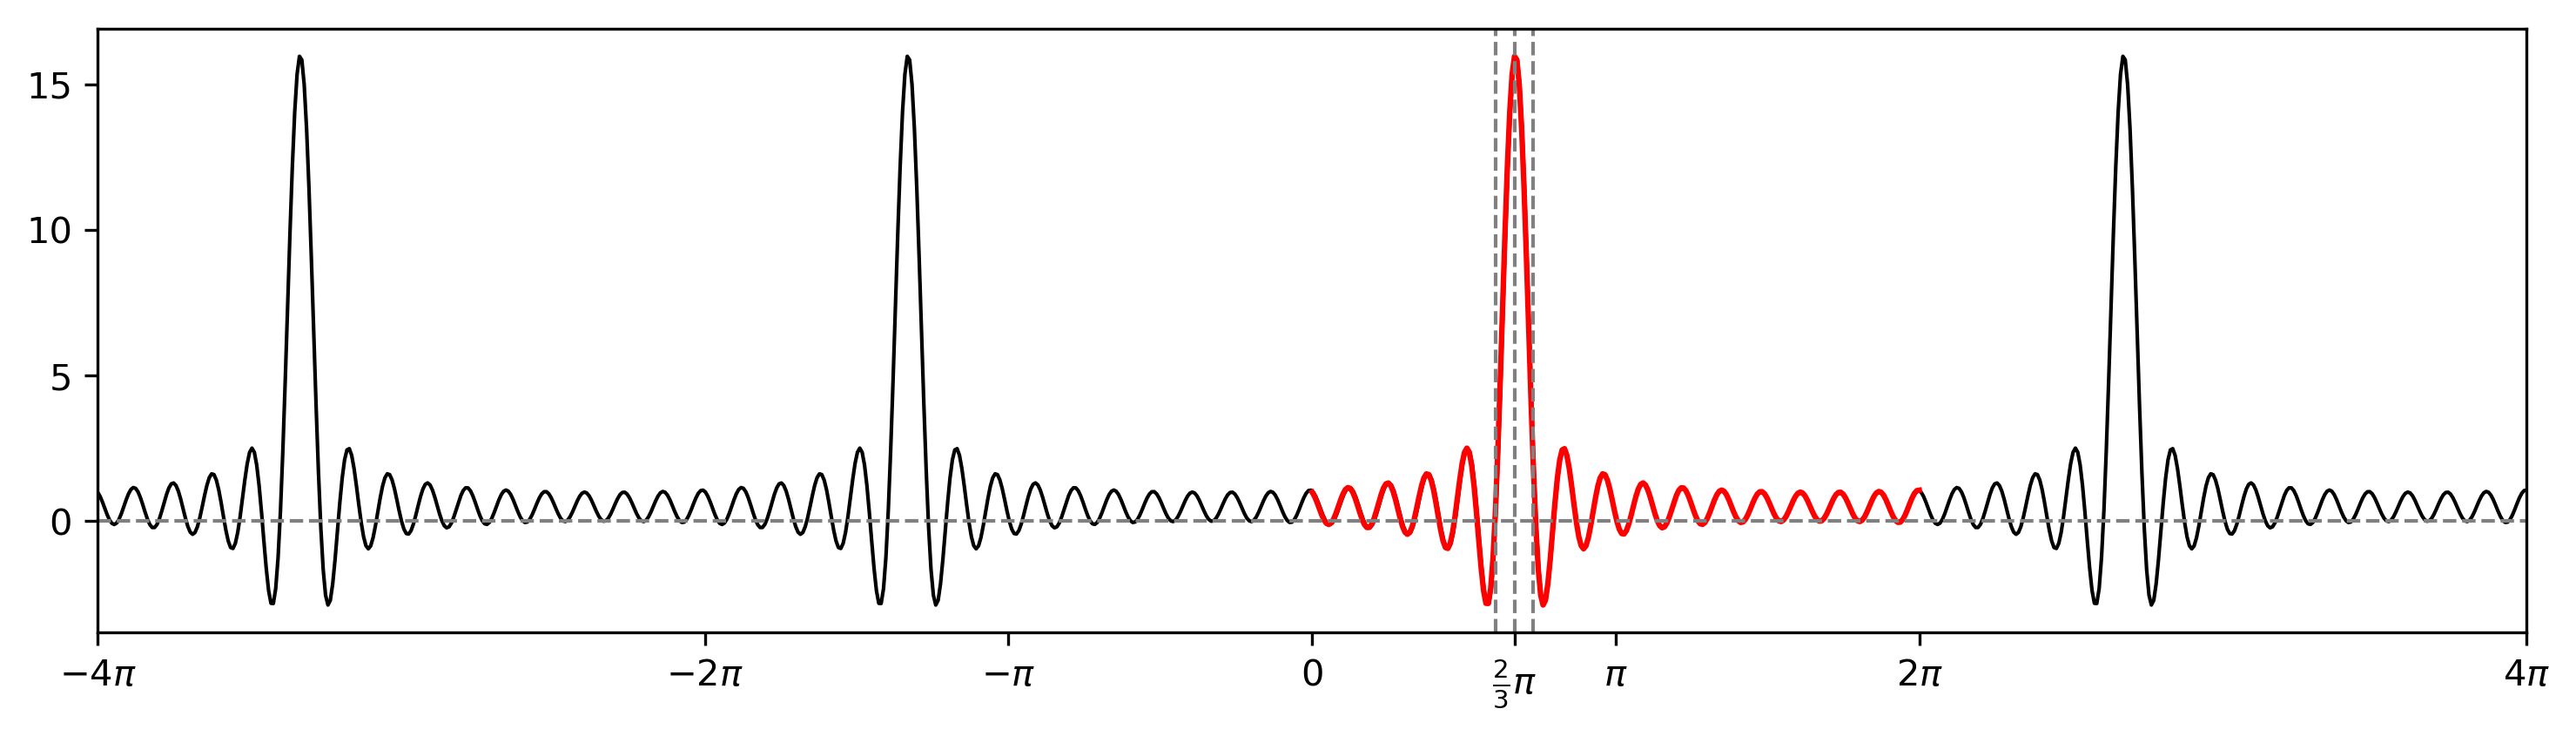
\includegraphics[width=6in]{external_image.png} 
    \fi
\end{figure}


\end{homeworkProblem}


%%%%%%%%%%%%%%%%%%%%%%%%%%%%%%%%%%%%%%%%%%%%%%%%%%%%
%%%%%%%%%%%%%%%%%%%%%%%%%%%%%%%%%%%%%%%%%%%%%%%%%%%%
%%%%%%%%%%%%%%%%%%%%%%%%%%%%%%%%%%%%%%%%%%%%%%%%%%%%
%%%%%%%%%%%%%%%%%%%%%%%%%%%%%%%%%%%%%%%%%%%%%%%%%%%%
    
\begin{homeworkProblem}[1.2]
    An example of tabular data.

    \begin{center}
    \begin{tabular}{l r}
    Sensor  & Arrival Time (ms) \\
    \hline
    0 & 4.50 \\
    1 & 4.25 \\
    2 & 4.00 \\
    3 & 3.75
    \end{tabular}
    \end{center}


\end{homeworkProblem}
        
        
%%%%%%%%%%%%%%%%%%%%%%%%%%%%%%%%%%%%%%%%%%%%%%%%%%%%
%%%%%%%%%%%%%%%%%%%%%%%%%%%%%%%%%%%%%%%%%%%%%%%%%%%%
%%%%%%%%%%%%%%%%%%%%%%%%%%%%%%%%%%%%%%%%%%%%%%%%%%%%
%%%%%%%%%%%%%%%%%%%%%%%%%%%%%%%%%%%%%%%%%%%%%%%%%%%%

\begin{homeworkProblem}[1.3]

    Can include source code listings using the \code{lstlisting} package. \\
    \code{https://en.wikibooks.org/wiki/LaTeX/Source\_Code\_Listings}

    The code can be written inline.
    \begin{lstlisting}[language=Python]
    import numpy as np
    180.0*np.arccos(0.1)/np.pi
    \end{lstlisting}

    Or included from an external file as in \ref{lst:external_example}.
    \lstinputlisting[language=Matlab, caption = {External File}, label=lst:external_example]{./external_file.m}

\end{homeworkProblem}

%%%%%%%%%%%%%%%%%%%%%%%%%%%%%%%%%%%%%%%%%%%%%%%%%%%%
%%%%%%%%%%%%%%%%%%%%%%%%%%%%%%%%%%%%%%%%%%%%%%%%%%%%
%%%%%%%%%%%%%%%%%%%%%%%%%%%%%%%%%%%%%%%%%%%%%%%%%%%%
%%%%%%%%%%%%%%%%%%%%%%%%%%%%%%%%%%%%%%%%%%%%%%%%%%%%

\begin{homeworkProblem}[1.5]
    \subsection{a)}
    An example of doing piece-wise expressions.
    \small
    \begin{align}
        \df{x_{1}} &= \begin{cases}
            1 & 0 \leq n \leq N-1 \\
            0 & otherwise
        \end{cases}
    \end{align}
    \normalsize
    
    \subsection{another subsection}
    Example of step by step derivation with explanation text.
    \small
    \begin{align}
        \ejO{X_{1}} &= \sum\limits_{n=0}^{N-1}e^{-j\Omega n} \\
        &= \frac{1-e^{-j\Omega N}}{1-e^{-j\Omega}} && \text{First N terms in geometric series} \\
        &= \frac{e^{-j\frac{\Omega N}{2}}\left[e^{j\frac{\Omega N}{2}}-e^{-j\frac{\Omega N}{2}}\right]\cdot2j}{e^{-j\frac{\Omega}{2}}\left[e^{j\frac{\Omega}{2}}-e^{-j\frac{\Omega}{2}}\right]\cdot2j} \\
        &= e^{-j\frac{\Omega N}{2}+\frac{\Omega}{2}}\frac{\sin\left(\frac{\Omega N}{2}\right)}{\sin\left(\frac{\Omega}{2}\right)} \\
        &= \frac{\sin\left(\frac{\Omega N}{2}\right)}{\sin\left(\frac{\Omega}{2}\right)}e^{-j\frac{\Omega}{2}\left(N-1\right)}
    \end{align}
    \normalsize

\end{homeworkProblem}
        
        
%%%%%%%%%%%%%%%%%%%%%%%%%%%%%%%%%%%%%%%%%%%%%%%%%%%%
%%%%%%%%%%%%%%%%%%%%%%%%%%%%%%%%%%%%%%%%%%%%%%%%%%%%
%%%%%%%%%%%%%%%%%%%%%%%%%%%%%%%%%%%%%%%%%%%%%%%%%%%%
%%%%%%%%%%%%%%%%%%%%%%%%%%%%%%%%%%%%%%%%%%%%%%%%%%%%

% Problem titles don't have to be numeric
\begin{homeworkProblem}[TWENTY]
    Some examples of helper commands for DSP expressions that I defined to reduce typing. (Plus an example of a footnote)
    \small
    \begin{align}
        \z{X} &= \cdots && \text{Z-transforms} \\
        \ejw{H} &= \cdots && \text{DTFT} \\
        \ejO{Y} &= \cdots && \text{DTFT with $\Omega$ instead of $\omega$} \\
        \nz{5} &= \cdots && \text{z to some power} \\
        \ejp{2\pi} &= \cdots && \text{positive powers of $e^{j}$} \\
        \ejn{2\pi} &= \cdots && \text{negative powers of $e^{j}$} \\
        \piover{2}{3} &= \cdots && \text{quick way to write fractions of $\pi$} \\
        \df{x} &= \cdots && \text{discrete signals} \\
        \dfd{x}{2} &= \cdots && \text{time shifted discrete signals} \\
        \dfn{x}{k} &= \cdots && \text{discrete signal with choice of index letter} \footnotemark
    \end{align}
    \normalsize
    \footnotetext{The code that defines these are in the preamble before the document begins. They are created using \code{newcommand}}

\end{homeworkProblem}
        
%%%%%%%%%%%%%%%%%%%%%%%%%%%%%%%%%%%%%%%%%%%%%%%%%%%%
%%%%%%%%%%%%%%%%%%%%%%%%%%%%%%%%%%%%%%%%%%%%%%%%%%%%
%%%%%%%%%%%%%%%%%%%%%%%%%%%%%%%%%%%%%%%%%%%%%%%%%%%%
%%%%%%%%%%%%%%%%%%%%%%%%%%%%%%%%%%%%%%%%%%%%%%%%%%%%

\begin{homeworkProblem}[5]
    Example of how to write a matrix
    \small
    \begin{align}
        M_{toeplitz} &= \begin{bmatrix}
        m_{0} & m_{-1} & m_{-2} & \cdots & m_{-n} \\
        m_{1} & m_{0} & m_{1} & \cdots & m_{-(n-1)} \\
        m_{2} & m_{1} & m_{0} & \cdots & m_{-(n-2)} \\
        \vdots & \vdots & \vdots & \ddots & \vdots \\
        m_{n} & m_{n-1} & m_{n-2} & \hdots & m_{0}
    \end{bmatrix}
    \end{align}
    \normalsize
\end{homeworkProblem}

%%%%%%%%%%%%%%%%%%%%%%%%%%%%%%%%%%%%%%%%%%%%%%%%%%%%
%%%%%%%%%%%%%%%%%%%%%%%%%%%%%%%%%%%%%%%%%%%%%%%%%%%%
%%%%%%%%%%%%%%%%%%%%%%%%%%%%%%%%%%%%%%%%%%%%%%%%%%%%
%%%%%%%%%%%%%%%%%%%%%%%%%%%%%%%%%%%%%%%%%%%%%%%%%%%%

\begin{homeworkProblem}[6]
    Probability helpers
    \small
    \begin{align}
        \E{X} &= \cdots && \text{Expected value using the proper capital E font} \\
        \Var{Z} &= \cdots && \text{Variance} \\
        x &\clsfr{b}{a} y && \text{Custom operator for bayes classifiers}
    \end{align}
    \normalsize
\end{homeworkProblem}

\end{document}
